\documentclass[12pt,letterpaper]{article}

% Paquetes esenciales
\usepackage[utf8]{inputenc}

\usepackage{amsmath, amssymb, amsthm}
\usepackage{graphicx} % Para insertar las gráficas de la Parte III
\usepackage{geometry}
\geometry{margin=2.5cm}
\usepackage{algorithm}
\usepackage{algpseudocode}
\usepackage{hyperref}
\usepackage{xcolor}

% Configuración de hipervínculos
\hypersetup{
    colorlinks=true,
    linkcolor=blue,
    urlcolor=blue
}

\begin{document}

% ==========================================
% ENCABEZADO
% ==========================================
\begin{center}
    {\Large \textbf{Universidad Nacional Autónoma de México}} \\[0.2cm] %
    {\large \textbf{Facultad de Ciencias}} \\[0.5cm] %
    {\large Análisis Matemático Aplicado} \\[0.2cm] %
    {\large Semestre 2026} \\[0.8cm] %
    {\Large \textbf{Tarea 5}} \\[0.5cm] %
    {\large \textbf{Nombre del la alumna:} [Karla Romina Juárez Torres]} \\[0.5cm]
\end{center}

\hrule
\vspace{1cm}

\subsection*{Ejercicio 1. Condición de Admisibilidad y Media Cero} %
\noindent Sea $\psi(t)\in L^{2}(\mathbb{R})$ una función wavelet madre. % 
La condición de admisibilidad que garantiza la existencia de la Transformada Ondicular Inversa está dada por: %
\begin{equation}
    C_{\psi}=\int_{-\infty}^{\infty}\frac{|\Psi(\omega)|^{2}}{|\omega|}d\omega<\infty %
\end{equation}
donde $\Psi(\omega)$ es la Transformada de Fourier de $\psi(t).$ % 
Demuestre analíticamente que, para que esta integral converja (y por tanto $C_{\psi}<\infty)$, es estrictamente necesario que la wavelet tenga media cero, es decir, $\int_{-\infty}^{\infty}\psi(t)dt=0.$ %

\vspace{0.5cm}
\noindent \textbf{Demostración:} \\
% Escribe tu demostración matemática aquí

Partamos de mantener finita a la constante $C_{\psi}$:
\begin{equation*}
    C_{\psi}=\int_{-\infty}^{\infty}\frac{|\Psi(\omega)|^{2}}{|\omega|}d\omega<\infty
\end{equation*}

La integral anterior tiene una posible singularidad justo en $\omega = 0$

Sabemos que $\psi(t) \in L^2(\mathbb{R})$, si además asumimos que decae lo bastante rápido como para pertenecer a $L^1(\mathbb{R})$, entonces su Transformada de Fourier $\Psi(\omega)$ va a ser una función continua si suponemos por un instante que $\Psi(0) \neq 0$, entonces podríamos tomar una vecindad muy pequeña $[-\epsilon, \epsilon]$ con centro en el origen y donde se cumpla que $|\Psi(\omega)|^2 \approx |\Psi(0)|^2 > 0$ asi si revisamos el comportamiento de la integral en es6to tenemos que
\begin{equation*}
    \int_{-\epsilon}^{\epsilon}\frac{|\Psi(\omega)|^{2}}{|\omega|}d\omega \approx |\Psi(0)|^{2} \int_{-\epsilon}^{\epsilon}\frac{1}{|\omega|}d\omega
\end{equation*}

Ahora la integral $\int_{-\epsilon}^{\epsilon}\frac{1}{|\omega|}d\omega$ tenemos que diverge de forma logarítmica. Así que, de suponer que $\Psi(0) \neq 0$, $C_{\psi}$ se nos iría a infinito y arruinaría por completo la condición de admisibilidad.

Así que para evitar esto necesitamos que el numerador anule esa singularidad osea
\begin{equation*}
    \Psi(0) = 0
\end{equation*}

Si tenemos en cuenta la definición clásica de la Transformada de Fourier para $\psi(t)$:
\begin{equation*}
    \Psi(\omega) = \int_{-\infty}^{\infty} \psi(t) e^{-i\omega t} dt
\end{equation*}

Y evaluamos directo en ($\omega = 0$), lo que nos queda es simplemente la integral de la señal en el dominio del tiempo 
\begin{equation*}
    \Psi(0) = \int_{-\infty}^{\infty} \psi(t) e^{-i(0) t} dt = \int_{-\infty}^{\infty} \psi(t) dt
\end{equation*}

Como ya vimos que $\Psi(0)$ tiene que ser cero entonces
\begin{equation*}
    \int_{-\infty}^{\infty} \psi(t) dt = 0
\end{equation*}
Con esto queda evidenciado que la función wavelet debe tener media cero. \hfill $\blacksquare$\vspace{1cm}


\subsection*{Ejercicio 2. Resolución en el Plano Tiempo-Frecuencia} %
\noindent Explique, utilizando el Principio de Incertidumbre de Heisenberg aplicado al procesamiento de señales $(\Delta t\cdot\Delta\omega\ge1/2)$, la diferencia fundamental entre el enventanado de la Transformada de Fourier a Corto Plazo (STFT) y el mecanismo de dilatación/compresión de la Transformada Ondicular Continua (CWT). %
¿Por qué la CWT es superior para analizar señales transitorias de alta frecuencia? %

\vspace{0.5cm}
\noindent \textbf{Respuesta:} \\
% Escribe tu justificación teórica aquí
Al aplicar este principio a señales nos encontramos con la desigualdad $\Delta t \cdot \Delta \omega \ge 1/2$ es decir no podemos ser infinitamente precisos al medir a la vez cuándo ocurre el evento que se estudie y qué frecuencias lo componen ya que siempre habrá un límite impuesto por lo anterior dicho

\textbf{Diferencias entre STFT y CWT:}
\begin{itemize}
    \item \textbf{STFT (Transformada de Fourier a Corto Plazo):} Utiliza una ventana de tamaño y forma inamovibles durante todo el proceso lo que hace rígidas las resoluciones $\Delta t$ y $\Delta \omega$ pero si afinamos la ventana para ubicar mejor los eventos en el tiempo tendriamos problemas para distinguir frecuencias similares y viceversa
    
    \item \textbf{CWT (Transformada Ondicular Continua):} Utiliza una \textit{wavelet madre} que se estira y encoge lo que nos da un margen totalmente dinamico así la \textit{wavelet} se ajusta de forma inversamente proporcional a la frecuencia que estemos analizando aunque se sigue respetando a Heisenberg y el área mínima de $\Delta t \cdot \Delta \omega$, lo que nos permite moldear sus dimensiones según lo que la señal nos exija en cada momento
\end{itemize}

\textbf{¿Por qué la CWT es mejor para atrapar transitorios de alta frecuencia?}

Notemos que los transitorioos suelen ser saltos bruscos que terminan pasando rapidamente es decir aportan altas frecuencias de golpe al espectro entonces CWT busca esas frecuencias altas usando parámetros de escala $a$ pequeñps y la wavelet se comprime en el tiempo lo que nos da una resolución dinamica y podemos hacer zoom en el tiempo, si intentáramos analizar esto con la STFT su ventana fija terminaría abarcando el transitorio y frecuencias de su alrededor dejándonos una idea borrosa de cuándo pasó realmente.\vspace{1cm}


\subsection*{Ejercicio 3. El Algoritmo de Cascada de Mallat (DWT)} %
\noindent El Análisis Multirresolución (MRA) nos permite calcular la Transformada Ondicular Discreta (DWT) en tiempo $\mathcal{O}(N)$ si nos apoyamos en un banco de filtros ortogonales. %

\vspace{0.5cm}
\noindent \textbf{1. Pseudocódigo de un nivel de descomposición DWT} %
% El algoritmo recibe S, g y h, y nos devuelve A y D tras aplicar convolución y diezmado

\begin{algorithm}[H]
\caption{Descomposición DWT - 1 Nivel}\label{alg:dwt1}
\begin{algorithmic}[1]
\Require Señal $S$ de longitud $N$, Filtro pasa-bajas $g$, Filtro pasa-altas $h$ de longitud $K$
\Ensure Coeficientes de Aproximación $A$, Coeficientes de Detalle $D$
\State $N \gets \text{longitud}(S)$
\State $K \gets \text{longitud}(g)$ \Comment{Asumimos que $g$ y $h$ miden lo mismo}
\State $M \gets \lfloor N / 2 \rfloor$ \Comment{La señal se reduce a la mitad después de diezmarla}
\State \textbf{Inicializar} arreglos $A$ y $D$ de tamaño $M$ llenos de ceros
\State \textbf{Convolución y Diezmado (Downsampling $\downarrow 2$):}
\For{$n \gets 0$ \textbf{to} $M - 1$}
    \For{$k \gets 0$ \textbf{to} $K - 1$}
        \If{$(2n - k) \ge 0$ \textbf{and} $(2n - k) < N$} \Comment{Para manejar los bordes / Zero-padding}
            \State $A[n] \gets A[n] + S[2n - k] \cdot g[k]$
            \State $D[n] \gets D[n] + S[2n - k] \cdot h[k]$
        \EndIf
    \EndFor
\EndFor
\State \Return $A, D$
\end{algorithmic}
\end{algorithm}

\vspace{0.5cm}
\noindent \textbf{2. Pseudocódigo para descomposición recursiva hasta el nivel $L$} %

\begin{algorithm}[H]
\caption{Descomposición DWT Recursiva (Nivel $L$)}\label{alg:dwtL}
\begin{algorithmic}[1]
\Require Señal original $S$, Nivel máximo $L$, Filtros $g$ y $h$
\Ensure Estructura con coeficientes $A_L$ y $D_1, D_2, \dots, D_L$
\State $A_{curr} \gets S$ \Comment{Al arrancar, nuestra aproximación es la señal tal cual}
\State $Detalles \gets \text{Lista vacía}$
\For{$nivel \gets 1$ \textbf{to} $L$}
    \State $A_{next}, D_{nivel} \gets \text{DWT\_1\_Nivel}(A_{curr}, g, h)$
    \State $Detalles.\text{agregar}(D_{nivel})$
    \State $A_{curr} \gets A_{next}$ \Comment{Pasamos los coef. de aproximación al siguiente nivel}
\EndFor
\State $A_L \gets A_{curr}$
\State \Return $A_L, Detalles$
\end{algorithmic}
\end{algorithm}

\vspace{1cm}


\subsection*{Ejercicio 4. El Escalograma (CWT)} %
El electrocardiograma que viene en la librería \texttt{scipy.misc} es el usado por que es un ejemplifica bien un tupo de señal no estacionaria

\vspace{0.5cm}
\noindent \textbf{1 y 2. Señal original en el dominio del tiempo} %

Calculo la CWT de la señal original del electrocardiograma usando una wavelet madre de Morlet

\begin{figure}[H]
    \centering
    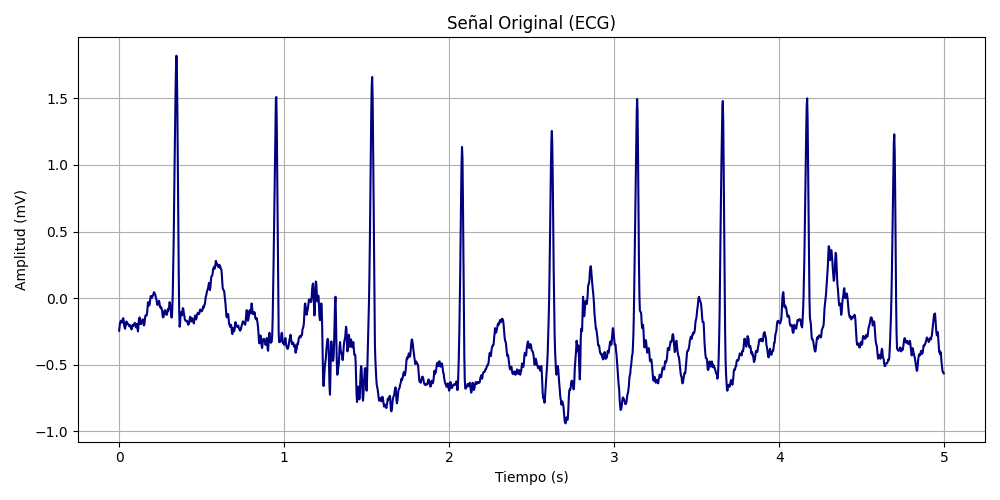
\includegraphics[width=0.8\textwidth]{figuras/ej4_senal_original.png} 
    \caption{Señal real de electrocardiograma no estacionaria.}
\end{figure}

\noindent \textbf{3. Escalograma Resultante} %

\begin{figure}[H]
    \centering
    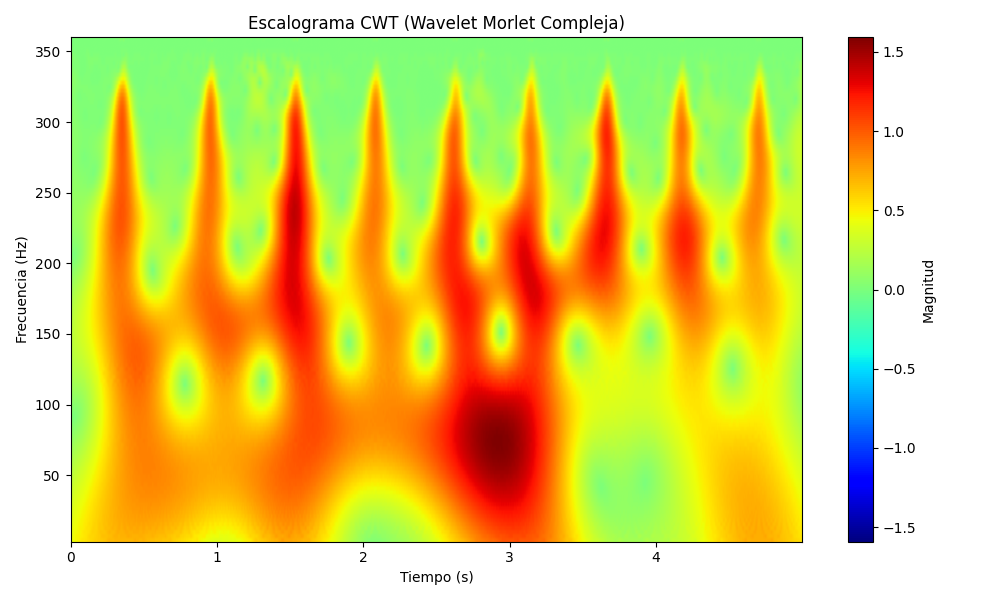
\includegraphics[width=0.8\textwidth]{figuras/ej4_escalograma.png} 
    \caption{Escalograma de la señal ECG utilizando wavelet de Morlet compleja Y es la frecuencia en Hz y el color indica la magnitud de los coeficientes.}
\end{figure}

\vspace{0.5cm}
\noindent \textbf{4. Identificación de eventos transitorios} %

Notemos que hay eventos transitorios que Fourier no mostraria
\begin{itemize}
    \item \textbf{Latido del corazón:} Aparece de forma periódica alrrededoir de 0.8 segundos que se ve en las franjas verticales muy intensas que van en frecuencias entre 10 Hz y 40 Hz notesé que el eje temporal se ven los picos del ECG 
    \item \textbf{Ondas P y T:} Antes y después de cada uno de estos complejos QRS se ven ven manchas aisladas de energía en frecuencias muy bajas que mustran cuando los ventrículos se despolarizan y repolarizan.
\end{itemize}

Si se tratara esto con un espectro de Fourier tradicional tendriamos que hay un montón de actividad entre 1 Hz y 40 Hz, pero no sabemos cuando latió el corazón. Pero, por otro lado el escalograma si nos muestra casi bastante precisamente cuándo ocurre cada pico y con qué frecuencias lo hace


\subsection*{Ejercicio 5. Denoising mediante Análisis Multirresolución (DWT)} %

Aqui le puse ruido gaussiano al electrocardiograma para simular como si la medición estuviera contaminada por algún equipo electrónico y con este me dediqué a limpiarla usando \textit{Wavelet Shrinkage}

Aproveché la Transformada Ondicular Discreta (DWT) con la familia ortogonal \textbf{Daubechies 4 (db4)}, llevándola hasta un nivel de descomposición $L=4$.

\begin{figure}[H]
    \centering
    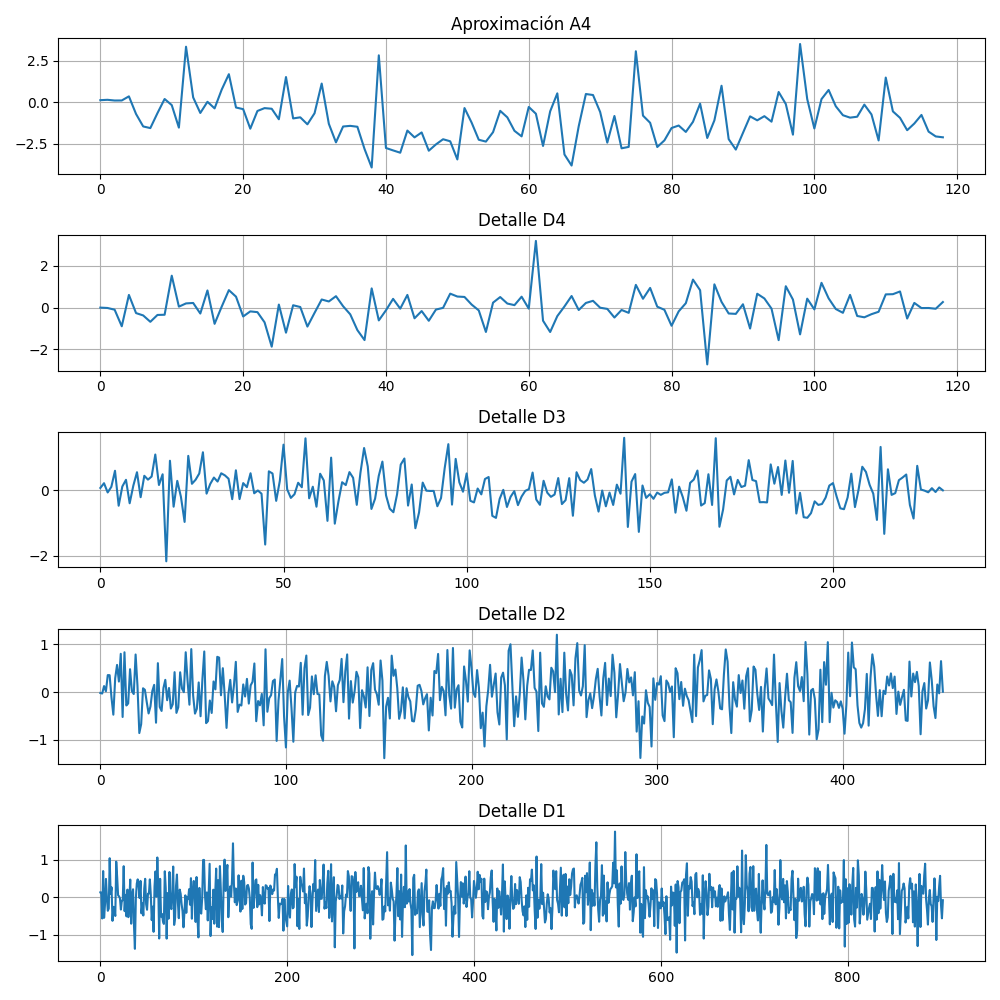
\includegraphics[width=0.8\textwidth]{figuras/ej5_coeficientes.png} 
    \caption{Cascada de coeficientes tras DWT (db4, Nivel 4): Aproximación $A_4$ y Detalles $D_4, D_3, D_2, D_1$.}
\end{figure}

Para quitar el ruido pasé todos los coeficientes desde $D_1$ hasta $D_4$ por una Soft Thresholding porque reduce un poco los coeficientes hacia cero
\begin{equation}
    D_{n}^{(soft)} = \text{sign}(D_n) \cdot \max(|D_n| - \lambda, 0)
\end{equation}

Y para el valor del umbral $\lambda$, decidí ocupar el VisuShrink
\begin{equation}
    \lambda = \sigma \sqrt{2 \ln N}
\end{equation}
Donde $N$ es la cantidad de muestras que tiene nuestra señal y $\sigma$ es lo que estimamos de desviación estándar para el ruido. 

Como en un caso real no sabria como es el ruido calculé la desviación estandar ocupando el Estimador Robusto de la Desviación Absoluta Mediana usando $D_1$
\begin{equation}
    \sigma = \frac{\text{mediana}(|D_1|)}{0.6745}
\end{equation}
El nivel $D_1$ casi toda la información que atrapamos es ruido gaussiano de alta frecuencia que inyectamos al principio, por lo que la constante solo sirve para calibrar el MAD y que funcione como un estimador para la distribución gaussiana

\vspace{0.5cm}
\noindent \textbf{4. Reconstrucción de la Señal (IDWT)} %

Como paso final, regresé al dominio del tiempo con la DWT inversa (IDWT). Para reconstruirla, junté los coeficientes de aproximación que dejamos intactos ($A_4$) con los de detalle que acababa de umbralizar.

\begin{figure}[H]
    \centering
    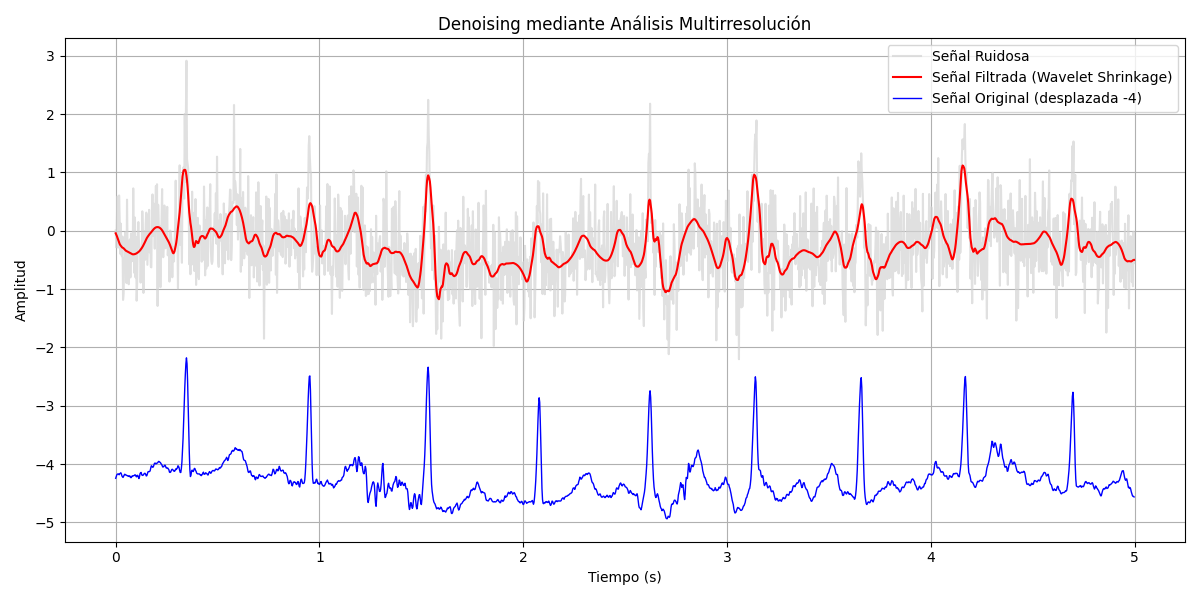
\includegraphics[width=1\textwidth]{figuras/ej5_denoising.png} 
    \caption{Superposición comparativa: Señal ruidosa, señal filtrada mediante Wavelet Shrinkage y la señal original (desplazada en el eje Y para mejor apreciación).}
\end{figure}

Notesé que es un filttrado bastante eficiente ya que si por otro lado se hubiera ocupado un filtro pasa-bajas de Fourier la señal se hubiera dejado irreconocible los picos de los latidos ya que se llevaría componentes de alta frecuencia que sí pertenecen al corazón y con Wavelet Shrinkage se conservan los bordes y transitorios tan marcados del electrocardiograma eliminando la estática


\end{document}